\documentclass[UKenglish]{ifimaster}
\usepackage[latin1]{inputenc}
\usepackage[T1]{fontenc,url}
\urlstyle{sf}
\usepackage{babel,textcomp,csquotes,duomasterforside,varioref,graphicx}
\usepackage[backend=biber,style=numeric-comp]{biblatex}
\usepackage{csvsimple}
\usepackage{booktabs}

\title{The title of my thesis}
\subtitle{Any short subtitle}
\author{Lucas Charpentier}

\bibliography{mybib}

\graphicspath{ {images/} }

\begin{document}
\duoforside[program={Computational Science},
    option={Imaging and Biomedical Computing},
    dept={Departement of Informatics \and Departement of Physics},
    long
    ]
\frontmatter{}
\maketitle{}

\chapter*{Abstract}
\tableofcontents{}
\listoffigures{}
\listoftables{}

\chapter*{Preface}

\mainmatter{}

\chapter{Introduction}
    \section{Background and Motivation}
    
    
    \section{Problem Statement}


    \section{Thesis Outline}


\chapter{Planning the project}
    \section{Machine Learning}
        \subsection{Supervised Learning}
        
        
        \subsection{Unsupervised Learning}

    
    \section{Artificial Neural Networks}
        \subsection{Perceptron}


        \subsection{Multilayer Perceptron}


        \subsection{Training a Neural Network}

    
    \section{Convolutional Neural Network}
        \subsection{Convolutional Layers}


        \subsection{Pooling Layers}

    
    \section{Neural Network Training Optimization}
        \subsection{Weight Initialization}


        \subsection{Training Batch Size}


        \subsection{Dropout}


    \section{Network Pruning}

    
    \section{Datasets}
        \subsection{MNIST}


        \subsection{Fashion MNIST}


        \subsection{CIFAR-10}


    \section{Architectures}
        \subsection{VGG-16}

\chapter{Single Layer ANN}
    In this chapter we will start by analyzing how effective removing nodes at random is. For this section we will only consider
    a single hidden layer ANN. We will then try estimating the importance of each node by using the loss function and classifying them
    as important, zero or worse. An important node is one that when removed would increase the loss of the model. A zero node will not
    significantly affect the loss of the model when removed. Lastly, a worse node will improve the loss of the model when removed. At
    this point we will also consider a 3 hidden layer MLP and a CNN with 4 convolutional layers followed by a dense layer in addition to
    the single layer ANN. By using these estimated node importance's, we still prune the models. We will start by pruning the models based
    on the pre-calculated node importance's, this will be slightly too extreme. Therefore, we will prune the networks by re-calculating
    the node importance's after removing a node till no node improves the model when removed. Initially, we will do this exhaustively by
    finding the node when removed will improve the model the most and then removing it. This is very time-consuming and we will therefore
    consider a "greedy" method that removes the first node that improves or does not affect the model, we will also start ignoring nodes
    that are quite important for the model in subsequent removals. For the sections on the pruning.


    TODO (Describe the datasets used, and the model we consider. Talk about the what we will keep the same during the whole project and what
    is kept the same for this chapter)
    \section{Pruning Nodes at Random}
        TODO - Describe the algorithms used to remove the nodes randomly

        \subsection{MNIST}
            Artificial Neural Network with single hidden layer of 128 nodes, using ADAM as optimizer with a learning rate of 0.001 trained on 5 epochs, batch size of 32.
            Final Accuracy and Loss on test set are:
            Loss: 0.0879
            Accuracy: 0.9724

            \begin{table}[h!]
                \centering
                \resizebox{\textwidth}{!}{\begin{tabular}{lrrrrrrr}
\toprule
{} &         1  &         2  &         4  &         8  &         16 &         32 &         64 \\
\midrule
count &  1000.0000 &  1000.0000 &  1000.0000 &  1000.0000 &  1000.0000 &  1000.0000 &  1000.0000 \\
mean  &     0.9720 &     0.9714 &     0.9704 &     0.9681 &     0.9619 &     0.9427 &     0.8485 \\
std   &     0.0009 &     0.0013 &     0.0020 &     0.0032 &     0.0056 &     0.0130 &     0.0417 \\
min   &     0.9687 &     0.9624 &     0.9602 &     0.9523 &     0.9270 &     0.8861 &     0.6831 \\
25\%   &     0.9715 &     0.9708 &     0.9694 &     0.9664 &     0.9588 &     0.9364 &     0.8215 \\
50\%   &     0.9721 &     0.9717 &     0.9708 &     0.9685 &     0.9628 &     0.9448 &     0.8546 \\
75\%   &     0.9726 &     0.9724 &     0.9719 &     0.9704 &     0.9660 &     0.9526 &     0.8803 \\
max   &     0.9736 &     0.9743 &     0.9744 &     0.9749 &     0.9724 &     0.9662 &     0.9328 \\
\bottomrule
\end{tabular}
}
                \caption[Short]{Long}
                \label{tab:ac_rnd_rem_mnist}
            \end{table}

            Trial text

            \begin{figure}[h!]\centering
                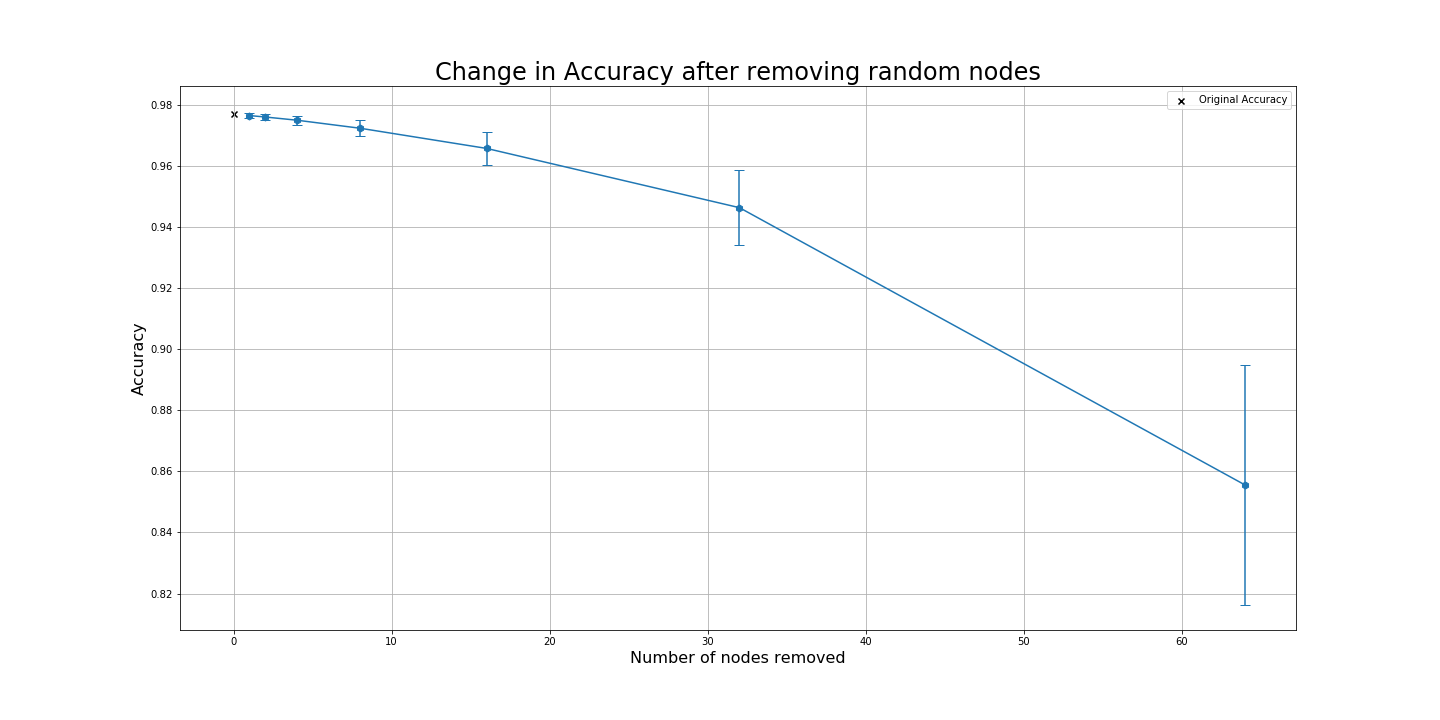
\includegraphics[width=\textwidth]{Accuracy_change_random_removal_mnist.png}
                \caption[Short title]{Testing}
                \label{fig:acc_rn_mnist}
            \end{figure}

            Trial text

            \begin{table}[h!]
                \centering
                \resizebox{\textwidth}{!}{\begin{tabular}{lrrrrrrr}
\toprule
{} &      1  &      2  &      4  &      8  &      16 &      32 &      64 \\
\midrule
\textbf{mean} &  0.0895 &  0.0914 &  0.0948 &  0.1024 &  0.1216 &  0.1794 &  0.4466 \\
\textbf{std } &  0.0026 &  0.0038 &  0.0058 &  0.0095 &  0.0164 &  0.0361 &  0.1074 \\
\textbf{min } &  0.0848 &  0.0839 &  0.0838 &  0.0844 &  0.0901 &  0.1127 &  0.2306 \\
\textbf{25\% } &  0.0877 &  0.0887 &  0.0907 &  0.0957 &  0.1101 &  0.1516 &  0.3662 \\
\textbf{50\% } &  0.0890 &  0.0907 &  0.0937 &  0.1012 &  0.1186 &  0.1738 &  0.4313 \\
\textbf{75\% } &  0.0908 &  0.0932 &  0.0981 &  0.1069 &  0.1305 &  0.1980 &  0.5112 \\
\textbf{max } &  0.0997 &  0.1245 &  0.1292 &  0.1489 &  0.2233 &  0.3409 &  0.9883 \\
\bottomrule
\end{tabular}
}
                \caption[Short]{Long}
                \label{tab:loss_rnd_rem_mnist}
            \end{table}

            Trial text

            \begin{figure}[h!]\centering
                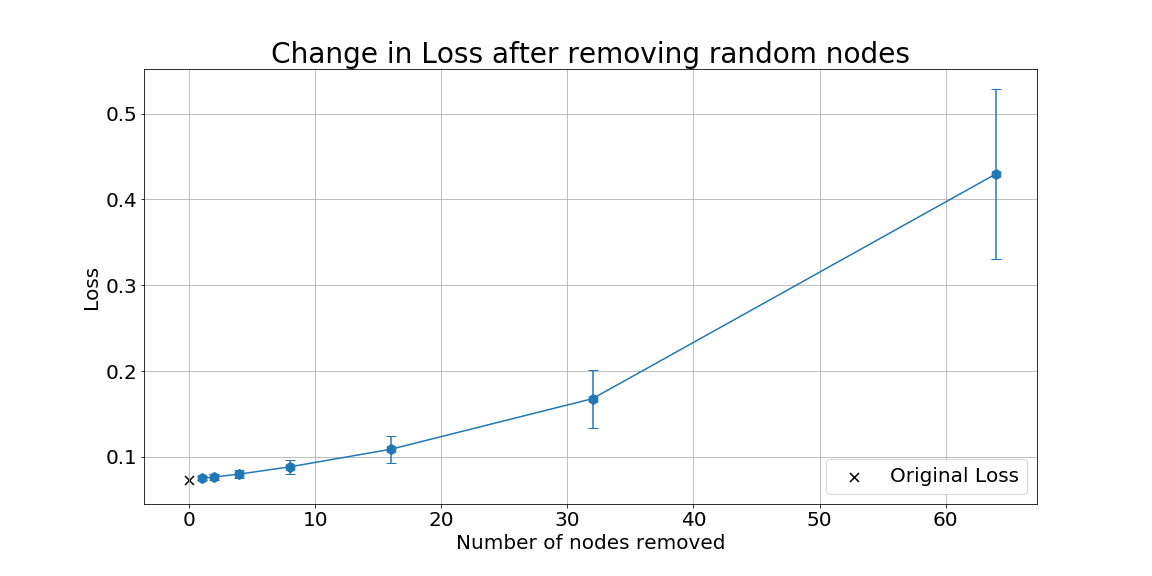
\includegraphics[width=\textwidth]{Loss_change_random_removal_mnist.png}
                \caption[Short title]{Testing}
                \label{fig:loss_rn_mnist}
            \end{figure}

            Trial text

            \begin{table}[h!]
                \centering
                \resizebox{\textwidth}{!}{\begin{tabular}{lrrrrr}
\toprule
{} &        1 &        2 &        3 &        4 &       8 \\
\midrule
\textbf{mean} &   7.4000 &   8.9000 &   8.2500 &   5.8000 &  2.4000 \\
\textbf{std } &   1.6983 &   2.7891 &   2.7314 &   3.3023 &  3.7613 \\
\textbf{min } &   5.0000 &   4.0000 &   3.0000 &   0.0000 &  0.0000 \\
\textbf{25\% } &   6.0000 &   7.5000 &   6.0000 &   4.0000 &  0.0000 \\
\textbf{50\% } &   7.0000 &   8.0000 &   9.0000 &   4.0000 &  0.0000 \\
\textbf{75\% } &   8.2500 &  10.0000 &   9.7500 &   8.0000 &  8.0000 \\
\textbf{max } &  11.0000 &  16.0000 &  12.0000 &  12.0000 &  8.0000 \\
\bottomrule
\end{tabular}
}
                \caption[Short]{Long}
                \label{tab:nr_rnd_rem_imp_mnist}
            \end{table}

            Trial text

            \begin{figure}[h!]\centering
                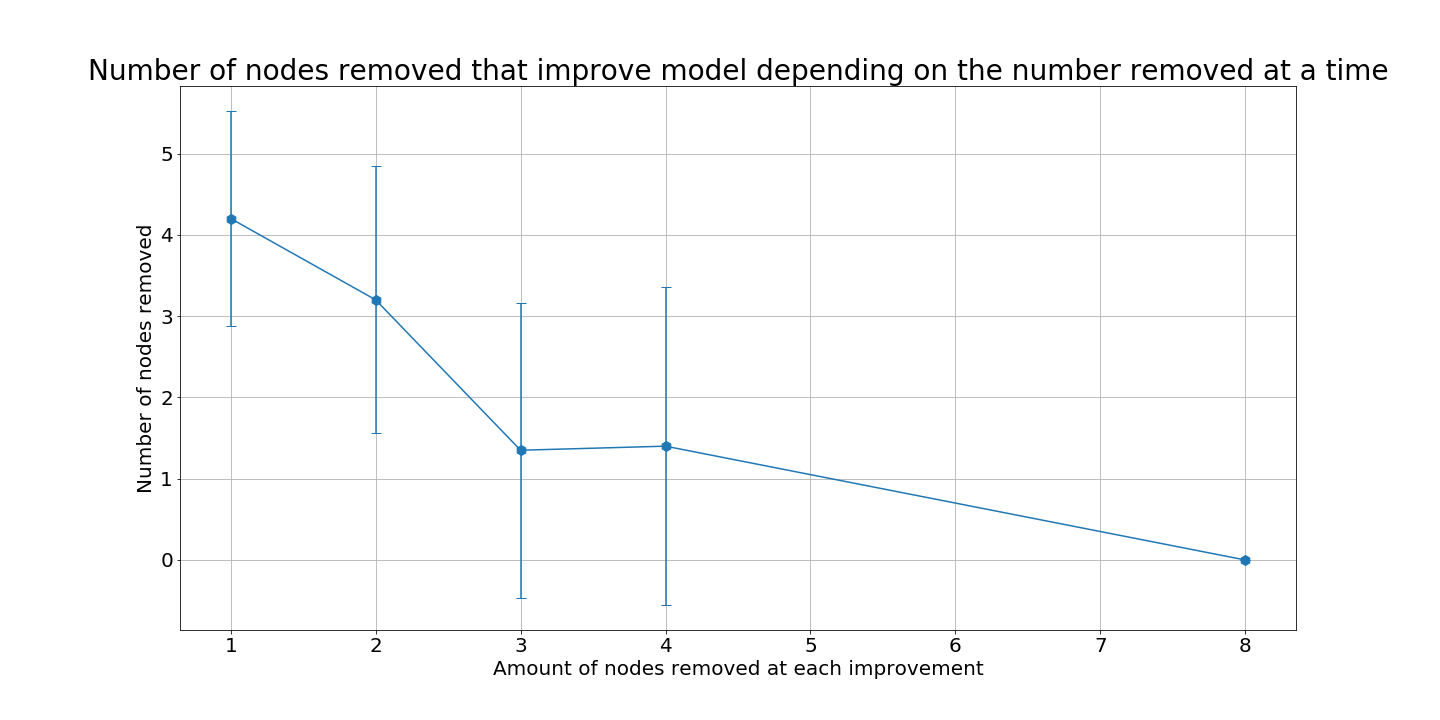
\includegraphics[width=\textwidth]{Num_rem_vs_size_removed_mnist.png}
                \caption[Short title]{Testing}
                \label{fig:num_rem_rn_imp_mnist}
            \end{figure}

            Trial text

            \begin{figure}[h!]\centering
                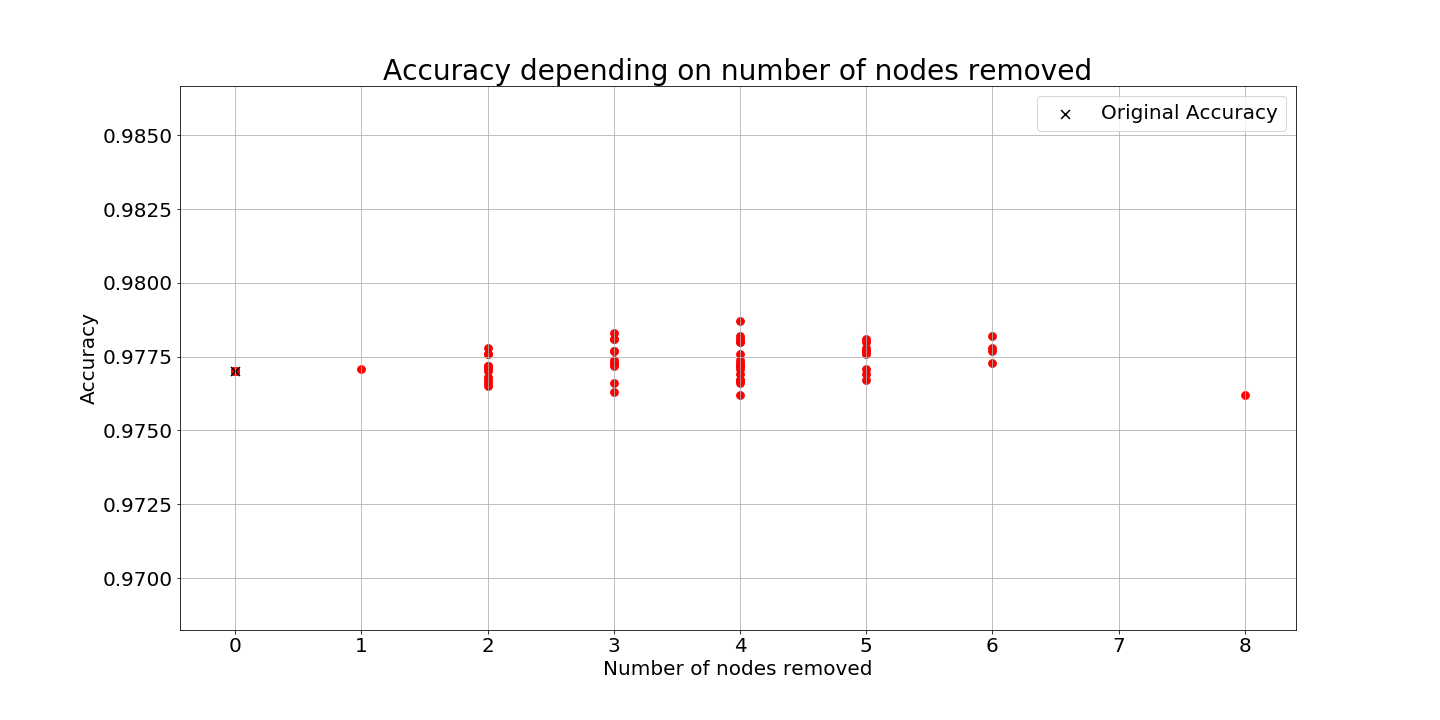
\includegraphics[width=\textwidth]{Accuracy_vs_nodes_removed_mnist.png}
                \caption[Short title]{Testing}
                \label{fig:acc_rn_imp_mnist}
            \end{figure}

            Trial text

            \begin{figure}[h!]\centering
                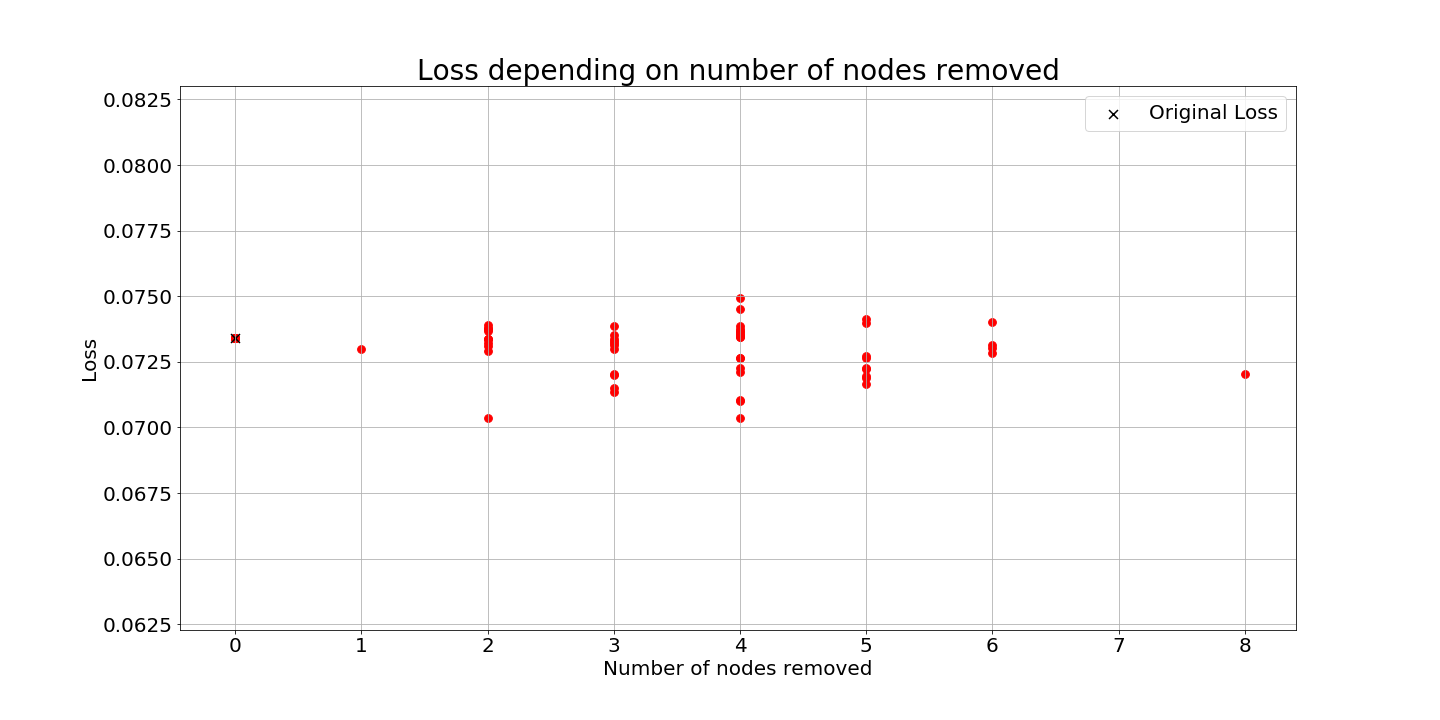
\includegraphics[width=\textwidth]{Loss_vs_nodes_removed_mnist.png}
                \caption[Short title]{Testing}
                \label{fig:loss_rn_imp_mnist}
            \end{figure}

            Trial text

        \subsection{Fashion MNIST}

            Trial text

            \begin{table}[h!]
                \centering
                \resizebox{\textwidth}{!}{\begin{tabular}{lrrrrrrr}
\toprule
{} &      1  &      2  &      4  &      8  &      16 &      32 &      64 \\
\midrule
\textbf{mean} &  0.8677 &  0.8667 &  0.8652 &  0.8618 &  0.8543 &  0.8295 &  0.7394 \\
\textbf{std } &  0.0021 &  0.0030 &  0.0042 &  0.0059 &  0.0096 &  0.0200 &  0.0443 \\
\textbf{min } &  0.8578 &  0.8470 &  0.8470 &  0.8405 &  0.8050 &  0.7382 &  0.5493 \\
\textbf{25\% } &  0.8670 &  0.8653 &  0.8632 &  0.8582 &  0.8491 &  0.8190 &  0.7171 \\
\textbf{50\% } &  0.8684 &  0.8674 &  0.8659 &  0.8626 &  0.8558 &  0.8336 &  0.7437 \\
\textbf{75\% } &  0.8686 &  0.8685 &  0.8681 &  0.8663 &  0.8611 &  0.8441 &  0.7698 \\
\textbf{max } &  0.8726 &  0.8735 &  0.8745 &  0.8767 &  0.8747 &  0.8656 &  0.8307 \\
\bottomrule
\end{tabular}
}
                \caption[Short]{Long}
                \label{tab:ac_rnd_rem_fmnist}
            \end{table}

            Trial text

            \begin{figure}[h!]\centering
                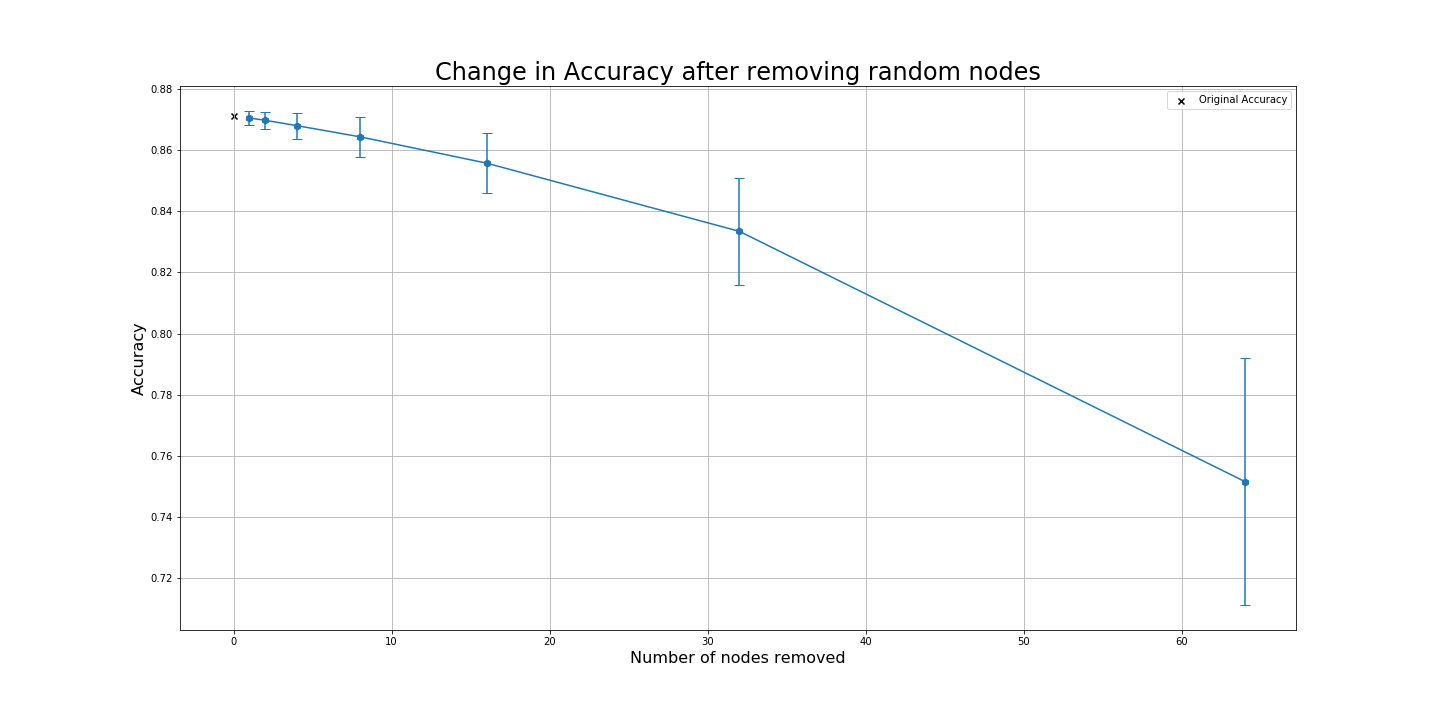
\includegraphics[width=\textwidth]{Accuracy_change_random_removal_fmnist.png}
                \caption[Short title]{Testing}
                \label{fig:acc_rn_fmnist}
            \end{figure}

            Trial text

            \begin{table}[h!]
                \centering
                \resizebox{\textwidth}{!}{\begin{tabular}{lrrrrrrr}
\toprule
{} &      1  &      2  &      4  &      8  &      16 &      32 &      64 \\
\midrule
\textbf{mean} &  0.3578 &  0.3601 &  0.3643 &  0.3730 &  0.3939 &  0.4607 &  0.7062 \\
\textbf{std } &  0.0049 &  0.0070 &  0.0098 &  0.0137 &  0.0228 &  0.0495 &  0.1182 \\
\textbf{min } &  0.3459 &  0.3452 &  0.3434 &  0.3448 &  0.3515 &  0.3725 &  0.4730 \\
\textbf{25\% } &  0.3557 &  0.3559 &  0.3576 &  0.3629 &  0.3772 &  0.4245 &  0.6235 \\
\textbf{50\% } &  0.3564 &  0.3584 &  0.3625 &  0.3711 &  0.3900 &  0.4504 &  0.6867 \\
\textbf{75\% } &  0.3591 &  0.3632 &  0.3693 &  0.3811 &  0.4060 &  0.4857 &  0.7619 \\
\textbf{max } &  0.3791 &  0.4055 &  0.4035 &  0.4297 &  0.5106 &  0.7079 &  1.3649 \\
\bottomrule
\end{tabular}
}
                \caption[Short]{Long}
                \label{tab:loss_rnd_rem_fmnist}
            \end{table}

            Trial text

            \begin{figure}[h!]\centering
                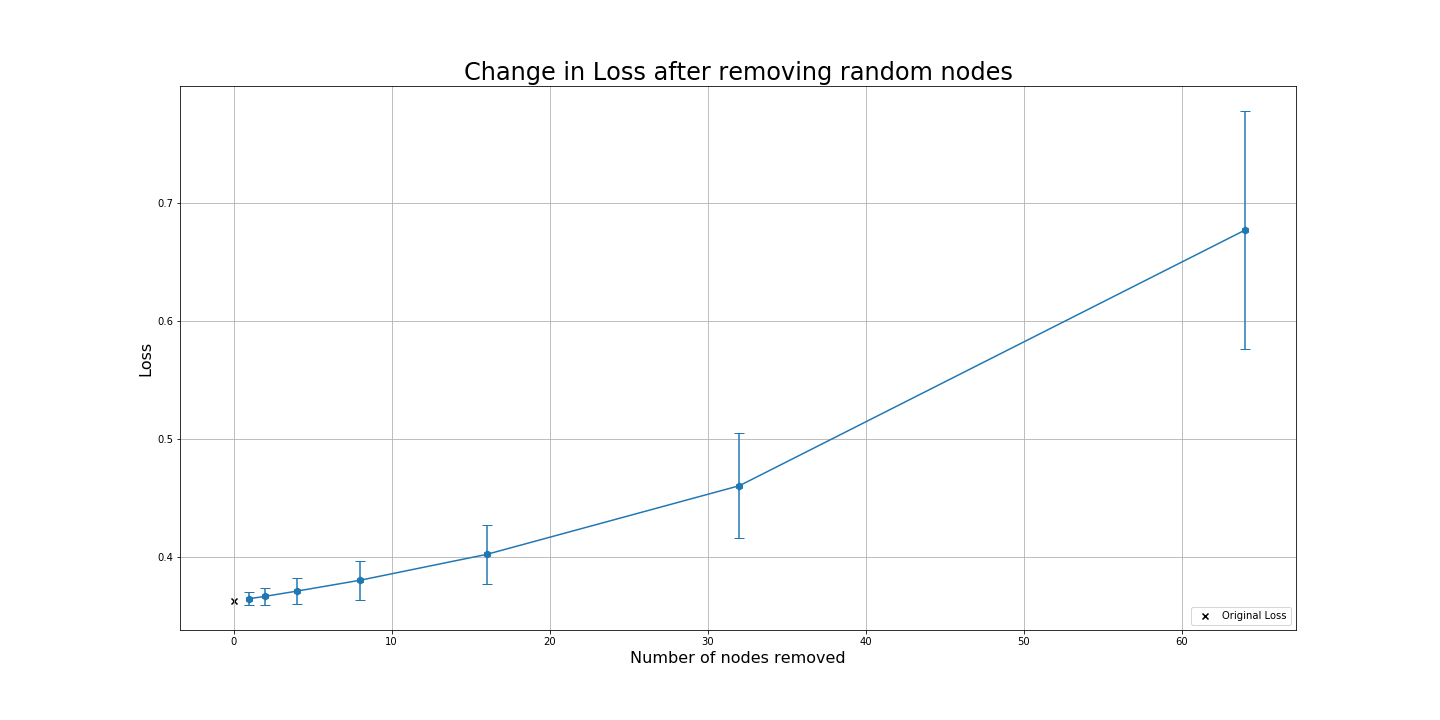
\includegraphics[width=\textwidth]{Loss_change_random_removal_fmnist.png}
                \caption[Short title]{Testing}
                \label{fig:loss_rn_fmnist}
            \end{figure}

            There is trial text here

            \begin{table}[h!]
                \centering
                \resizebox{\textwidth}{!}{\begin{tabular}{lrrrrr}
\toprule
{} &       1 &        2 &        3 &       4 &       8 \\
\midrule
\textbf{mean} &  5.5000 &   8.6000 &  10.6500 &   8.400 &  5.6000 \\
\textbf{std } &  1.5728 &   1.8468 &   3.1502 &   3.409 &  3.7613 \\
\textbf{min } &  2.0000 &   6.0000 &   3.0000 &   4.000 &  0.0000 \\
\textbf{25\% } &  5.0000 &   8.0000 &   9.0000 &   7.000 &  0.0000 \\
\textbf{50\% } &  5.5000 &   8.0000 &  12.0000 &   8.000 &  8.0000 \\
\textbf{75\% } &  6.2500 &  10.0000 &  12.0000 &  12.000 &  8.0000 \\
\textbf{max } &  8.0000 &  12.0000 &  18.0000 &  16.000 &  8.0000 \\
\bottomrule
\end{tabular}
}
                \caption[Short]{Long}
                \label{tab:nr_rnd_rem_imp_fmnist}
            \end{table}

            Trial text

            \begin{figure}[h!]\centering
                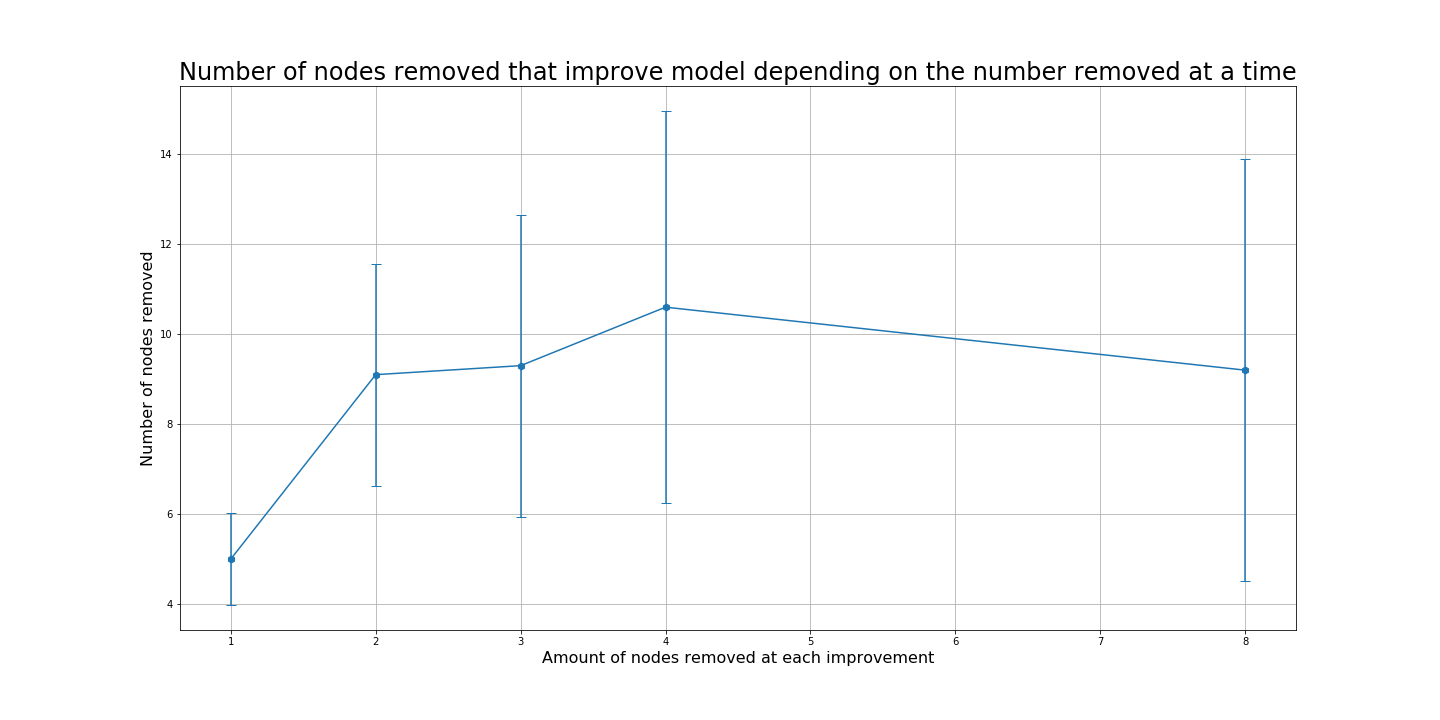
\includegraphics[width=\textwidth]{Num_rem_vs_size_removed_fmnist.png}
                \caption[Short title]{Testing}
                \label{fig:num_rem_rn_imp_fmnist}
            \end{figure}

            Trial text

            \begin{figure}[h!]\centering
                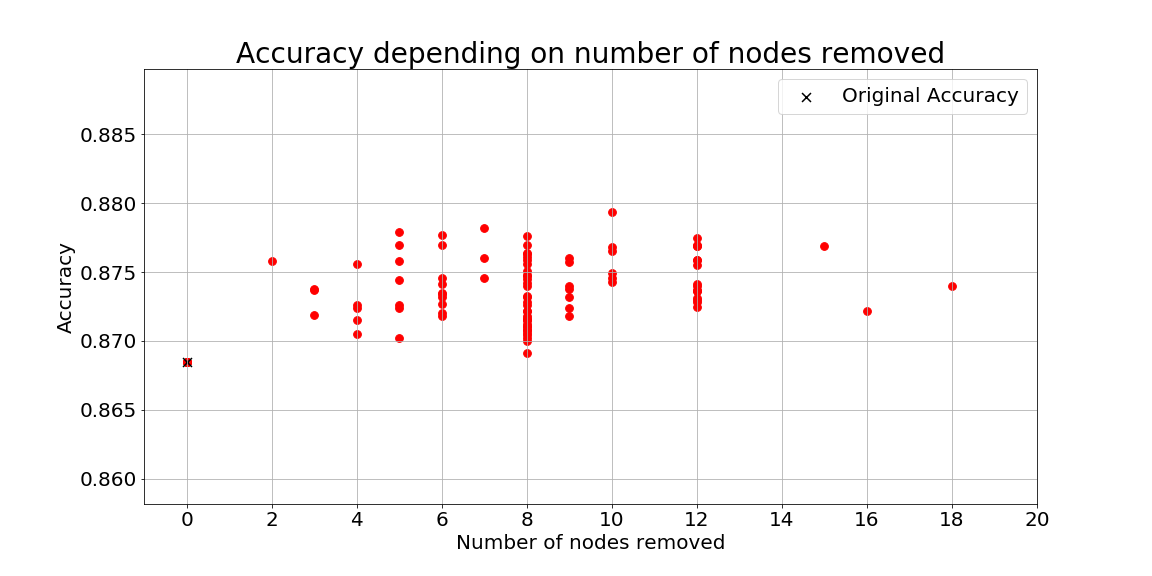
\includegraphics[width=\textwidth]{Accuracy_vs_nodes_removed_fmnist.png}
                \caption[Short title]{Testing}
                \label{fig:acc_rn_imp_fmnist}
            \end{figure}

            Trial text

            \begin{figure}[h!]\centering
                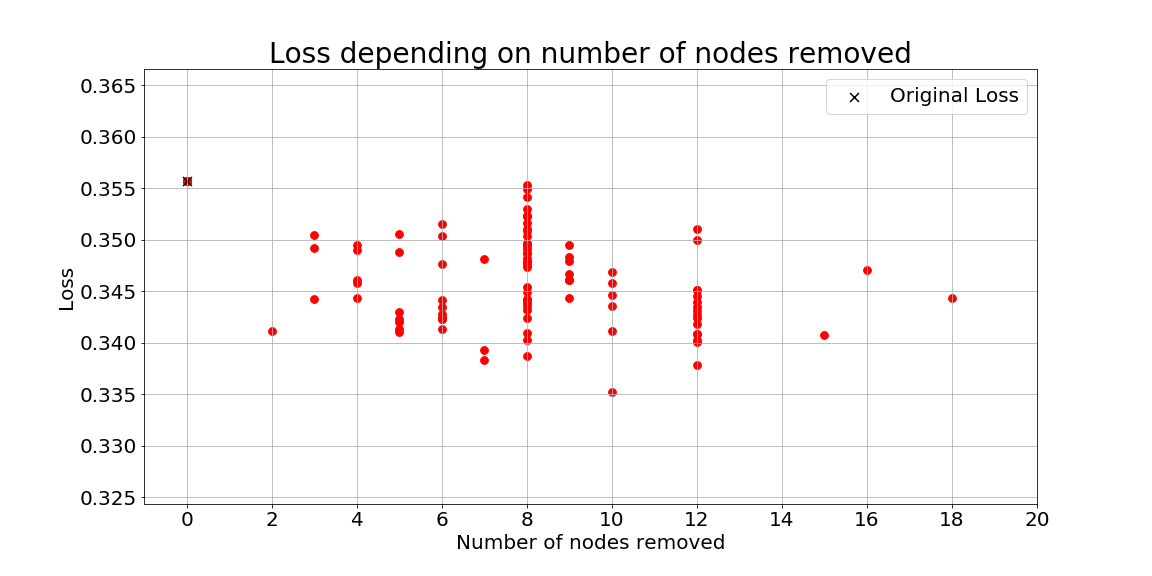
\includegraphics[width=\textwidth]{Loss_vs_nodes_removed_fmnist.png}
                \caption[Short title]{Testing}
                \label{fig:loss_rn_imp_fmnist}
            \end{figure}

            Trial text

    \section{Estimating Node Importance based on Loss}
        TODO - Describe the algorithms used

    \section{Pruning network with pre-calculated importance}
        TODO - Describe the algorithms used

    \section{Pruning Nodes based on the Loss}
        TODO - Describe the algorithms used

    \section{Greedy approach to pruning instead of Exhaustive approach}
        TODO - Describe the algorithms used

\chapter{Multi-Layer Perceptron}
    \section{Effects of Changing Training Batch Size on Node Importance}


    \section{Effects of Using Dropout}


    \section{Iterative weight initialization using Node importance}



\chapter{Convolutional Neural Network}
    \section{Looking at effects of per class accuracy after pruning}


    \section{Pruning based on class accuracy}


\chapter{Case study: Reducing a VGG-16 model trained on X dataset}

\chapter{Conclusion}
    \section{Summary}


    \section{Future Works}


\backmatter{}
\printbibliography
\end{document}